\documentclass[12pt]{article}

\usepackage[utf8]{inputenc}
\usepackage{amsmath, amssymb}
\usepackage{geometry}
\usepackage{hyperref}
\usepackage{graphicx}
\usepackage{fancyhdr}
\usepackage{hyperref}
\usepackage{float}
% Page layout
\geometry{a4paper, margin=1in}

% Header and footer
\pagestyle{fancy}
\fancyhf{}
\fancyhead[L]{Real-Time Systems}
\fancyhead[R]{\thepage}
\setlength{\headheight}{14.49998pt} % Adjust head height
\addtolength{\topmargin}{-2.49998pt} % Compensate for the increased head height
\hypersetup{
    colorlinks,
    linkcolor=black,
    filecolor=black,      
    urlcolor=cyan,
}
% Title
\title{Appunti sistemi embedded \\ Scheduling in Real-Time Systems}
\author{}
\date{2025}

\begin{document}

\maketitle
\tableofcontents
\newpage
\section{Introduzione}

I sistemi real time sono sistemi di computazione dove la reazione a eventi dell'ambiente deve avvenire entro precisi requisiti temporali.
Dunque la correttezza della computazione non dipende unicamente dal risultato prodotto, ma anche dal tempo in cui il risultato è prodotto.
Una reazione ritardata potrebbe essere inutile o addirittura dannosa.
Molto spesso questi sistemi vengono implementati attraverso la programmazione in assembly o con driver a basso livello per la gestione delle periferiche, manipolazione delle task 
e la priorità degli interrupt.
\\
Questo approccio presenta degli svantaggi
\begin{itemize}
    \item Programmazione tediosa
    \item Codice poco comprensibile
    \item Difficile manutenibilità
    \item Difficile verifica dei vincoli temporali
\end{itemize}
La conseguenza maggior di questo approccio è che il software costruito tramite tecniche empiriche può  essere impredicibile.\\
Se tutti i vincoli temporali critici non possono essere verificati a priori e il sistema operativo non include meccanismi specifici per maneggiare i task real-time
il sistema potrebbe apparentemente funzionare correttamente per un certo periodo di tempo, ma potrebbe fallire in situazioni particolari.
Il testing, pur essendo importante, non può essere una soluzione per ottenere la predicibilità in un sistema real-time. Questo vale perché 
il flusso di controllo dipende anche da eventi esterni dell'ambiente, che non possono essere interamente inclusi nel testing.
\section{Real time}
La correttezza del sistema non dipende solamente dal risultato logico prodotto dalla computazione ma anche dal tempo in cui il risultato è prodotto.
Il termine reale indica che la reazione del sistema a eventi esterni deve avvenire \textbf{durante} la loro evoluzione.
Di conseguenza il tempo interno al sistema deve essere misurato usando la stessa scala utilizzata per misurare il tempo dell'ambiente controllato.
Al livello di processo la principale differenza tra un task real-time e non è la presenza di una \textbf{deadline}, ovvero il tempo massimo in cui una task deve essere completata.
In un sistema critico una task che non rispetta la deadline non solo è in ritardo, è anche un errore!
In base alle conseguenze a cui porta il non rispettare la deadline le task possono essere suddivise in:
\begin{itemize}
\item \textbf{Hard} se il non rispetto della deadline porta a conseguenze catastrofiche, ad esempio il fallimento di un sistema di controllo di un aereo.
\item \textbf{Firm} se il non rispetto della deadline porta a un output inutile al sistema ma non produce conseguenze catastrofiche.
\item \textbf{Soft} se il non rispetto della deadline porta a una degradazione della qualità del servizio ma non produce conseguenze catastrofiche.
\end{itemize}
Un sistema in grado di gestire task hard real-time è detto \textbf{hard real-time system}.
Alcuni di questi sistemi sono tendenzialmente sistemi \textbf{safety critical}.
\subsection{Limiti dei sistemi real-time correnti}
Molti dei sistemi attualmente in uso sono soluzioni basate su kernel, che sono versioni modificate di sistemi operativi a time sharing.
Una conseguenza di questo è che condividono le stesse feature di base dei sistemi a time sharing, che non sono adatte a sistemi real-time.
Le caratteristiche principali sono:
\begin{itemize}
\item \textbf{Multitasking}\\
    Supporto per la programmazione concorrente offerta attraverso un insieme di chiamate a sistema per la gestione dei processi. Molte di queste primitive
    non prendono in considerazione il tempo e, peggio ancora, introducono ritardi senza limiti ai tempi di esecuzione, il che potrebbe portare le task hard a non rispettare le deadline in maniera non predicibile.
\item \textbf{Scheduling basato su priorità}\\
    Meccanismo flessibile di scheduling, dato che permette di implementare diverse strategie in base alla maniera in cui assegno le priori
    Nonostante ciò, mappare i constraint a un insieme di priorità è difficile e non sempre possibile, specialmente in un sistema dinamico.
    Il problema principale è che i kernel permettono un \textbf{numero limitato di livelli di priorità}, mentre le deadline possono variare molto di più.
    In sistemi dinamici l'arrvo di una nuova task può comportare un remappaggio dell'intero insieme di priorità.
\item \textbf{Capacità di rispondere velocemente agli interrupt}\\
    Solitamente questa feature viene ottenuta tramite la possibilità di impostare una priorità per gli interrupt, più alta rispetto alla priorità dei processi e 
    riducendo al minimo le porzioni di codice eseguite con le interruzioni disabilitate.
    \\
    Nota che questo approccio aumenta la reattività del sistema agli eventi esterni, ma introduce dei ritardi non limitati all'esecuzione dei processi.
    Infatti, un processo di un'applicazione sarà sempre interrotto da un interrupt di un driver, anche se è più importante che venga servita la periferica.
\item \textbf{Meccanismo di base per la comunicazione tra processi e sincronizzazione}\\
    Tipicamente semafori binari per la sincronizzazione e la mutua esclusione su risorse condivise.
    Però, se nessun protocollo d'accesso è utilizzato per entrare in sezioni critiche i semafori possono generare una serie di problemi, ad esempio la \textbf{priority inversion} o deadlokc.
\item \textbf{Small kernel e context switch veloce}\\
    Questa feature riduce l'overhead del sistema, dunque migliora il response time medio dell'insieme di task. 
    Ciò nonostante non è sufficiente per garantire il rispetto delle deadline. D'altro canto un kernel piccolo implica limitate funzionalità, il che ha effetto sulla predicibilità del sistema.
\item \textbf{Supporto a clock real-time come reference di tempo interna}\\
    Feature essenziale di ogni kernel real-time che gestisce task hard real-time che interagiscono con l'ambiente esterno.
    Nella maggior parte dei kernel commerciali questo è l'unico meccanismo di temporizzazione disponibile.
    In molti casi non vi sono primitive per controllare esplicitamente i constraint temporali delle task, e non c'è un supporto per l'attivazione automatica delle task periodiche.
\end{itemize}
La mancanza di una qualsiasi garanzia preclude l'utilizzo di questi sistemi in casi in cui i requisiti temporali siano stringenti.
\subsection{Feature desiderabili di un sistema real-time}
La predicibilità può essere ottenuta apportando pesanti modifiche ai tipici sistemi a time sharing.
Alcune proprietà importanti sono:
\begin{itemize}
\item \textbf{Timeliness}\\
    I risultati non devono essere corretti solo nel loro valore ma anche nel dominio temporale.
    Di conseguenza il sistema operativa deve fornire degli specifici meccanismi del kernel per la gestione del tempo e 
    per la gestione dei task con constraint temporali espliciti e criticità diverse.
\item \textbf{Predicibilità}\\\
    Per raggiungere il livello di performance desiderato, il sistema deve essere analizzabile per prevedere le conseguenze di ogni decisione di scheduling.
    Nelle applicazioni safety critical tutti i requisiti temporali devono esser garantiti a priori, prima di mettere il sistema in azione.
    Se qualche vincolo non può essere garantito, il sistema deve essere in grado di informare l'utente e delle decisioni alternative devono essere prese.
\item \textbf{Efficienza}\\
    La maggior parte dei sistemi real-time sono embedded, dunque l'efficienza è un requisito fondamentale.
\item \textbf{Robustezza}\\
    Il sistema deve essere in grado di continuare a funzionare a qualsiasi condizioni di carico. La gestione dell'overload e il comportamento di adattamento sono feature essenziali per sistemi con molta varianza di carico.
\item \textbf{Tolleranza agli errori}\\
    Singoli errori hardware o software non devono portare a un fallimento del sistema.
\item \textbf{Manutenibilità}\\
    L'architettura di un sistema real-time deve essere progettata in maniera modulare per permettere di eseguire modifiche facilmente.
\end{itemize}
\section{Fonti di impredicibilità}
Un sistema dovrebbe essere in grado di prevedere l'evoluzione delle task e garantire in anticipo che tutti i vincoli temporali critici 
vengano rispettati.
L'affidabilità della garanzia dipende da un insieme di fattori, che includono anche le caratteristiche fisiche dell'hardware e 
i meccanismi/politiche del kernel.
\\
La prima componente che influisce sulla predicibilità è il processore. Le caratteristiche del processore, ad esempio il prefetch delle istruzioni, 
pipelining, cache, DMA sono fonti di \textbf{non determinismo}.
\\
Pur aumentando le performance medie del sistema, introducono fattori di non determinismo che prevengono una precisa stima dei worst-case-execution-time (WCETs).
Altre caratteristiche che influenzano la predicibilità sono le caratteristiche interne del kernel, come l'algoritmo di scheduling, i meccanismi di sincronizzazione, 
i tipi di semafori, le politiche di gestione della memoria e le politiche di gestione degli interrupt.
\subsection{DMA}
Uno dei modi più comuni per implementarlo è tramite cycle stealing, il DMA controller prende il controllo del bus per un ciclo di clock 
e poi lo rilascia al processore.
Durante l'operazione di DMA il trasferimento e l'esecuzione del codice sul processore avvengo in parallelo.
SE la CPU e il DMA controller richiedono un ciclo di memoria allo stesso tempo, il bus viene assegnato al DMA controller e la CPU
aspetta finché il DMA non ha finito.
In questo modo non è possibile prevedere il tempo di esecuzione di un task, dato che il tempo di esecuzione dipende da quante volte il DMA controller ha bisogno del bus.
\\
Una possibile soluzione al problema è il time slicing, dove un ciclo di memoria è diviso in due slot di tempo adiacenti, uno per il DMA e uno per la CPU.
Questa soluzione è più costosa ma più prevedibile di cycle stealing, dato che il response time di una task non è influenzato dal DMA.
\subsection{Cache}
Nei sistemi real-time la cache è una fonte di non determinismo, dato che il tempo di accesso alla memoria dipende dalla presenza o meno del dato in cache.
Quando avviene un cache miss il tempo di accesso alla memoria è molto più lungo, e questo non è prevedibile.
Quando si effettua una scrittura in memoria l'utilizzo della cache risulta costoso perché il tempo di accesso alla memoria è più lungo, dato che deve essere garantita la consistenza.
\subsection{Interrupts}
Un grosso problema per la predicibilità è la gestione degli interrupt provenienti dalle periferiche I/O.
Se non gestite correttamente possono introdurre ritardi non limitati durante l'esecuzione di processi.\\
In quasi tutti i sistemi operativi la gestione di un interrupt prevede l'esecuzione di una service routine dedicata per la gestione del device.
Il vantaggio di questo metodo è che tutti i dettagli hardware sono contenuti nel driver.\\
In molti OS gli interrupt vengono serviti usando un sistema a priorità fissa, tramite i quali ogni driver viene schedulato in base a una priorità statica, questa priorità è più alta rispetto a quella di qualsiasi processo.
In generale è molto difficile prevedere a priori il numero di interrupt che un task può ricevere, dunque il delay è impredicibile.
\\
Per ridurre l'interferenza dei driver sui task ed effettuare operazioni di I/O le periferiche devono essere gestiste differentemente
\subsubsection{Approccio A}
La soluzione più radicale è disattivare tutti gli interrupt esterni, a eccezione di quelli generati dal timer.
Tutte le periferiche vanno gestiste dall'applicazione (controllo di programma), i quali hanno accesso ai registri delle periferiche.
Dato che non ci sono più interrupt, il trasferimento deve essere effettuato tramite polling.
L'accesso diretto alle periferiche consente alta flessibilità al livello di programma ed elimina i delay introdotti dai driver.
Dunque il tempo necessario per un trasferimento può essere calcolato a priori.
Un altro vantaggio è che il kernel non va modificato quando una nuova periferica viene aggiunta o ne viene rimossa una.
\\
Lo svantaggio principale è che risulta poco efficiente dato la busy wait necessaria per il polling.
Un grosso problema è che le applicazioni richiedono la conoscenza completa dei dettagli a basso livello delle periferiche che devono gestire.
Questo può essere gestito incapsulando le routine che dipendono dai device in una libreria.
\subsubsection{Approccio B}
Come nella soluzione precedente tutti gli interrupt esterni sono disabilitati,
tranne quelli dei timer.\\
In questa soluzione le periferiche non vengono gestite direttamente dall'applicazione, ma a turno da routine dedicate del kernel 
periodicamente attivate dal timer.
Questo approccio elimina i ritardi causati dai driver e confina le operazioni di I/O a una o più routine periodiche del kernel.
In alcuni sistemi i device I/O vengono suddivisi in due gruppi in base alla loro velocità, quelli più veloci vengono gestiti da task 
periodici con frequenza maggiore.
\\
Il vantaggio di questo metodo è che tutti i dettagli hardware sono incapsulati nel kernel, dunque l'applicazione non ha bisogno di 
conoscere i dettagli a basso livello delle periferiche.
Dato che gli interrupt sono disabilitati il maggior problema è dato dalla busy wait delle procedure di gestione dell'I/O del kernel.
Questo metodo introduce un overhead maggiore rispetto all'approccio A, richiede modifiche al kernel quando una periferica viene aggiunta o rimossa.
\subsubsection{Approccio C}
Lasciare gli interrupt abilitati e ridurre al minimo possibile i driver per le periferiche.
L'unico scopo dei driver è quello di attivare una task che gestisce il device. Una volta attivato il task di gestione del device 
viene eseguito sotto diretto controllo del sistema operativo
ed è schedulato come un task normale.
In questo modo la priorità che può essere assegnata al task di gestione del device è completamente indipendente dalle altre priorità 
può essere impostata in base ai requisiti del programma.
\begin{figure*}[h]
\centering
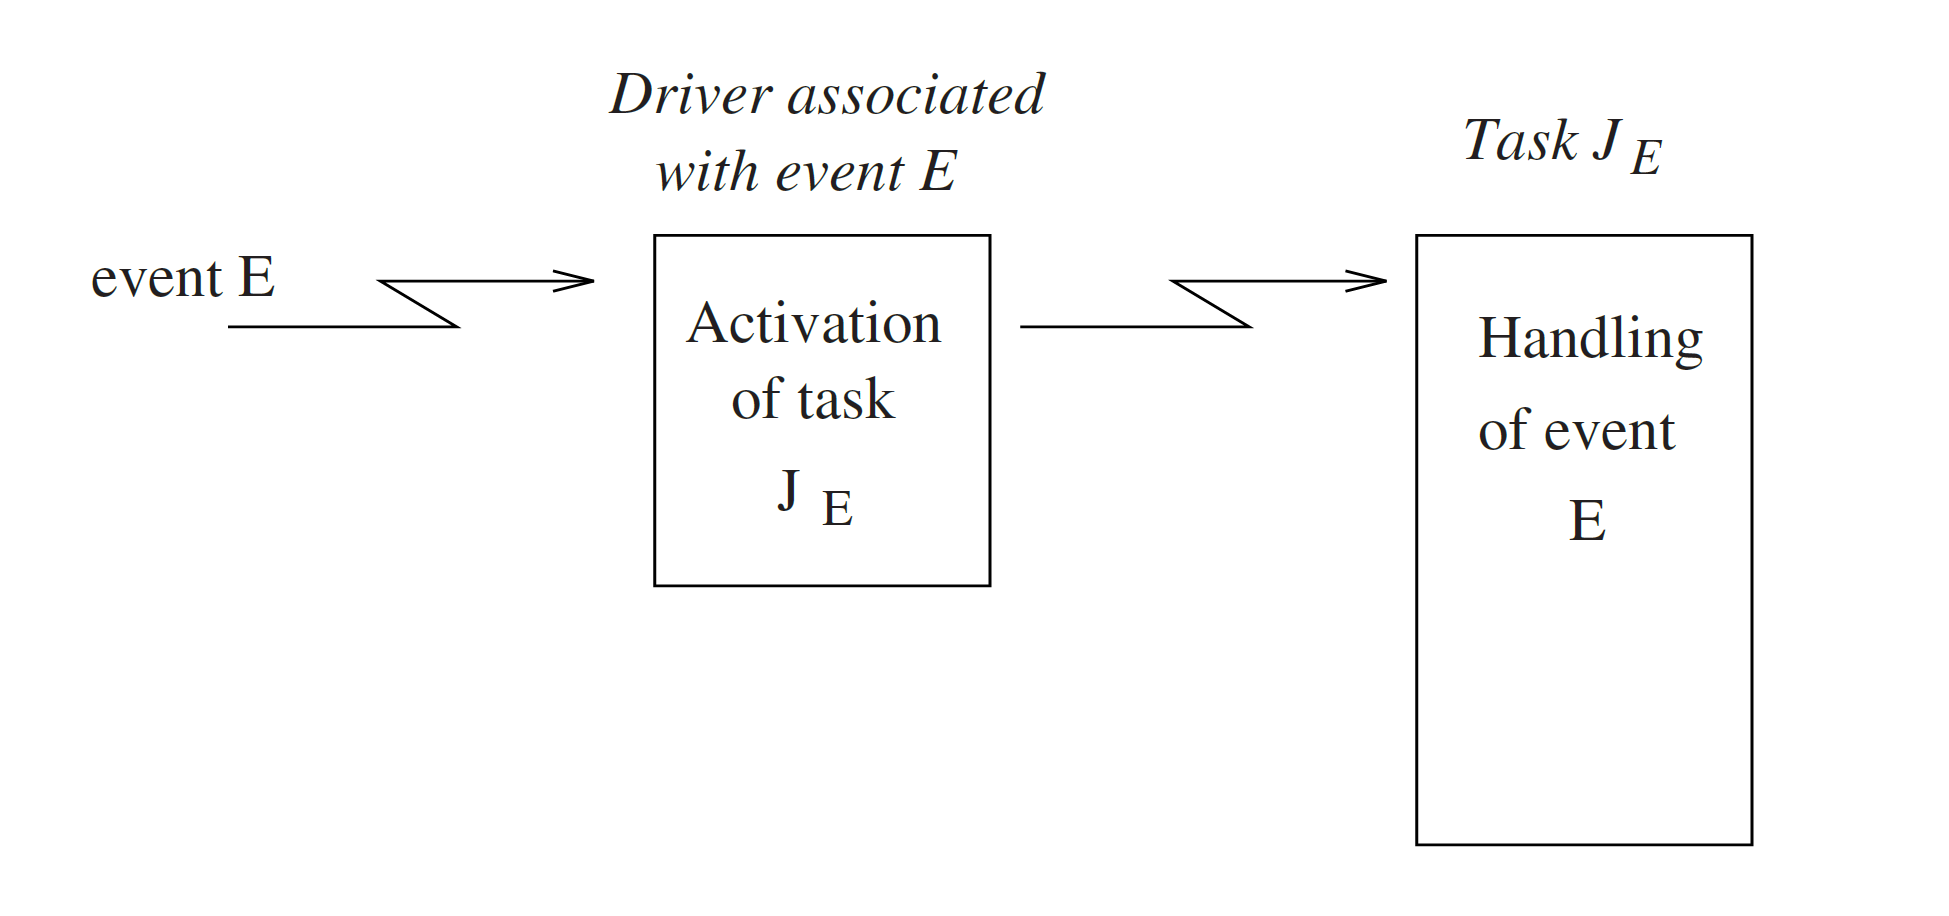
\includegraphics[height=150px]{pictures/approccioC.png}
\caption{Attivazione task per la gestione del device}
\end{figure*}
\\
Il vantaggio principale di questo metodo è che il busy wait viene eliminato e il tempo di esecuzione del driver di gestione del device è 
molto ridotto, di conseguenza il tempo di esecuzione del task è più prevedibile.
Nella maggior parte delle applicazioni pratiche il piccolo overhead portato da questo tipo di driver viene ignorato.

\subsection{Semafori}
L'usuale meccanismo dei semafori utilizzato nei sistemi operativi tradizionali non è adatto per i sistemi real-time per via del fenomeno dell'\href{https://en.wikipedia.org/wiki/Priority_inversion}{inversione di priorità}.
L'inversione di priorità deve essere evitato a tutti i costi in un sistema real-time, dato che introduce non determinismo sull'esecuzione di task critiche.
Per quanto riguarda il problema della mutua esclusione l'inversione di priorità può essere evitata usando protocolli specifici che devono essere usati ogni 
volta che si effettua un accesso alla sezione critica.
L'implementazione di questo tipo di protocollo potrebbe richiedere estensive modifiche al kernel, che non comprendono solo le primitive $wait$ e $signal$, ma anche strutture dati e meccanismi di task management.
\subsection{Gestione della memoria}
Come gli altri aspetti del kernel, la gestione della memoria deve essere progettata per evitare il non determinismo.
Ad esempio sistemi di paging on-demand non sono adatti a sistemi con rigidi vincoli temporali a causa dei lunghi e imprevedibili ritardi causati dalle page fault e page replacement.
LE soluzioni tipiche adottate nei sistemi real-time prevedono regole di segmentazione della memoria con uno schema fisso. Il partizionamento statico è particolarmente efficace quando i programmi richiedono
una quantità di memoria simile tra loro.
In generale gli schemi di allocazione statici aumentato la predicibilità del sistema, ma diminuiscono la flessibilità in sistemi dinamici, dunque la scelta progettuale va fatta bilanciando le due caratteristiche.
\subsection{Linguaggi di programmazione}
Con l'aumentare della complessità dei sistemi real-time aumenta anche la necessità di utilizzare astrazioni offerte dai linguaggi.
\\
Purtroppo i linguaggi attualmente a disposizioni non sono abbastanza espressivi da permettere di esprimere certi comportamenti temporali, dunque non sono adatti per la programmazione di sistemi real-time.
L'esistenza di costrutti che modificano il flusso di controllo del programma in maniera non deterministica, come gli $if$, rende impossibile la stima affidabile dei WCETs in attività concorrenti.
Un'altra fonte di impredicibilità è data dalla ricorsione, l'analizzatore di scheduling non è in grado di prevedere il numero di chiamate ricorsive e il tempo di esecuzione.

\section{Concetti di base di scheduling}
\subsection{Introduzione}
Un \textbf{processo} è una computazione eseguita dalla CPU in maniera sequenziale, d'ora in poi useremo il termine processo come sinonimo di \textit{task} o \textit{thread}.
\\
In realtà un processo è una entità più complessa composta da vari task (o thread)
che condividono lo stesso spazio di indirizzamento e le stesse risorse.
Una \textbf{politica di scheduling} è un criterio secondo il quale la CPU viene assegnata ai vari task che si sovrappongono.
L'insieme di politiche che in ogni istante di tempo determinano l'ordine con il quale i task vengono eseguiti è detto \textbf{algoritmo di scheduling}.\\
L'operazione specifica di assegnare la CPU a un task selezionato dall'algoritmo di scheduling è detta \textbf{dispatching}.
Quando un processo può essere potenzialmente eseguito dalla CPU, possiamo avere due casi: 
\begin{itemize}
    \item Il processo è in \textbf{running} perché è già stato selezionato dall'algoritmo di scheduling e la CPU è stata assegnata a lui.
    \item Il processo è in \textbf{ready} e aspetta di essere selezionato dall'algoritmo di scheduling.
\end{itemize}
In entrambi i casi il processo viene detto un task \textbf{attivo}. Tutti i processi in wait vengono tenuti in una \textbf{ready queue}. I vari sistemi operativi possono utilizzare anche più code dipendentemente dal tipo di task.
\begin{figure}
\centering
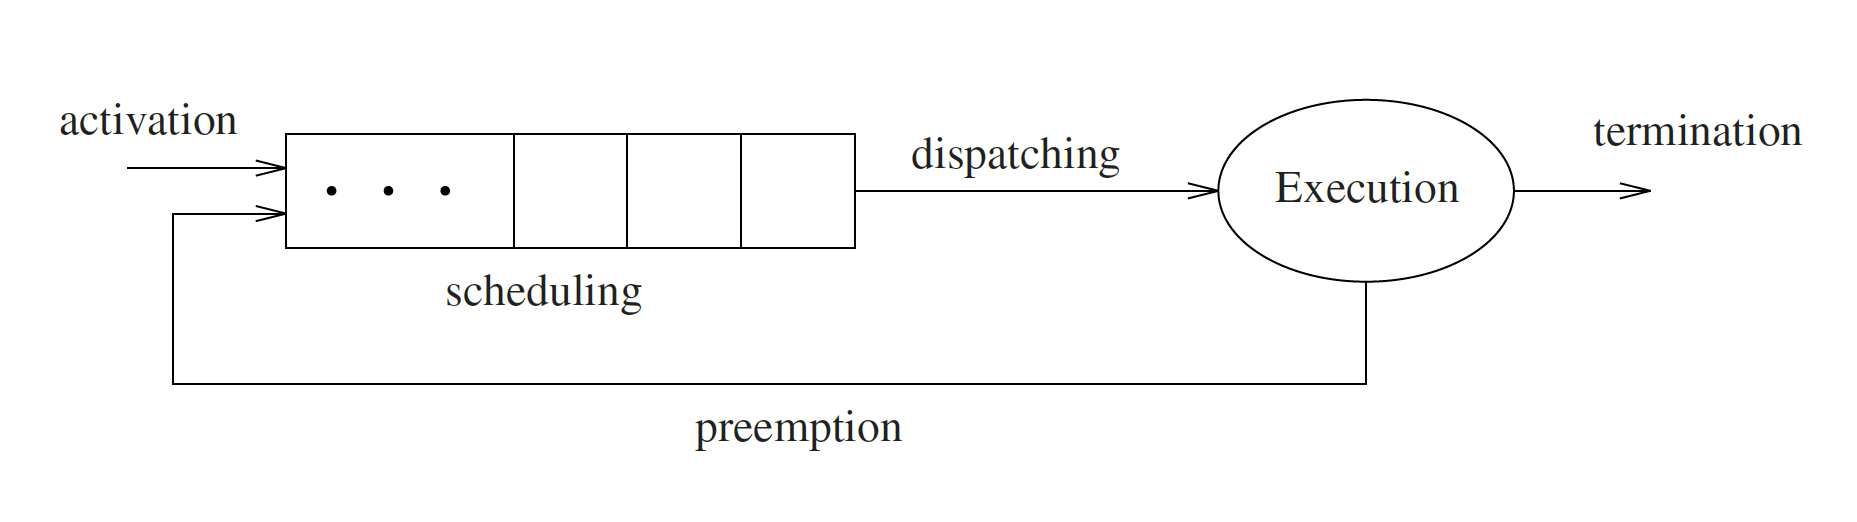
\includegraphics[width=\textwidth]{pictures/cicloEsecuzione.png}
\caption{Coda di task in ready che aspettano di essere eseguiti}
\end{figure}
In molti sistemi dove è concessa l'attivazione dinamica dei task, questi possono essere interrotti in qualsiasi momento, così che quando un task più importante entra nel sistema esso possa essere eseguito immediatamente senza aspettare nella ready queue.
L'operazione di interrompere il task in esecuzione e reinserirlo nella ready queue è detta \textbf{preemption}.\\
Nei sistemi real-time la preemption è importante per 3 motivi:
\begin{itemize}
    \item I task che gestiscono le eccezioni potrebbero aver bisogno di fare preemption di task in esecuzione per garantire che le eccezioni siano gestite in tempo.
    \item Quando i task hanno livelli di priorità diversi, i task critici possono essere eseguiti immediatamente.
    \item Tipicamente lo scheduling con preemption permette maggiore efficienza, nel senso che permette l'esecuzione di task real time con una percentuale di utilizzo di CPU maggiore.
\end{itemize}
D'altro canto la preemption distrugge la località dei programmi e introduce overhead, di conseguenza limitare la preemption in un sistema real-time può essere benefico.
\\
Uno schedule è detto \textbf{feasible} se tutti i task possono essere eseguiti rispettando l'insieme di vincoli a essi posti.
Un insieme di task è detto \textbf{schedulabile} se esiste uno schedule che rispetta i vincoli di tutti i task.
\subsection{Tipi di vincoli di scheduling}
Tipicamente i vincoli applicabili a task real time rientrano in tre classi:
\begin{itemize}
    \item Vincoli temporali
    \item Vincoli di precedenza
    \item Vincoli di mutua esclusione su risorse condivise
\end{itemize}
\subsubsection{Vincoli temporali}
I sistemi realtime sono caratterizzati da attività computazionali con stringenti vincoli temporali che devono essere rispettati per ottenere il comportamento desiderato.
Un requisito tipico è che un task deve essere completato entro un certo tempo, detto \textbf{deadline}.\\
Se la deadline è rappresentata in rispetto a quando il task è stato attivato, essa è detta \textbf{relative deadline}, altrimenti è detta \textbf{absolute deadline}.\\
In base alle conseguenze a cui porta il non rispetto della deadline le task possono essere suddivise in:
\begin{itemize}
    \item \textbf{Hard} se il non rispetto della deadline porta a conseguenze catastrofiche, ad esempio il fallimento di un sistema di controllo di un aereo.
    \item \textbf{Firm} se il non rispetto della deadline porta a un output inutile al sistema ma non produce conseguenze catastrofiche.
    \item \textbf{Soft} se il non rispetto della deadline porta a una degradazione della qualità del servizio ma non produce conseguenze catastrofiche.
\end{itemize}
\begin{figure}[h]
    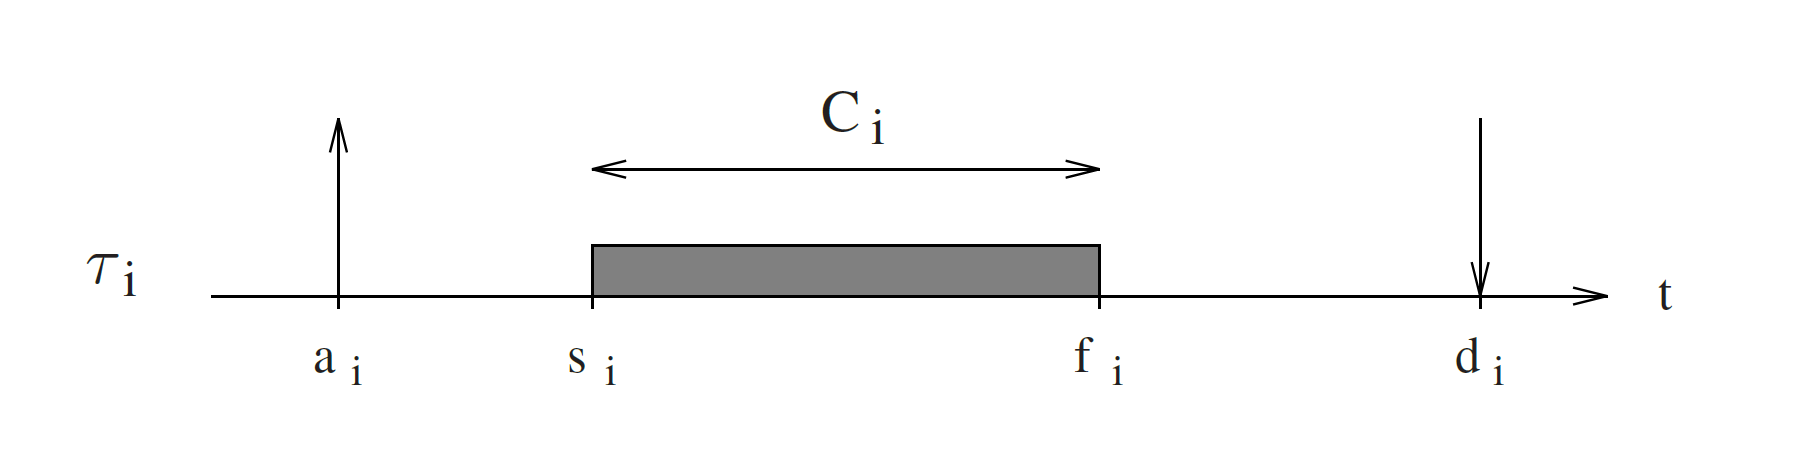
\includegraphics[width=\textwidth]{pictures/parametriTask.png}
    \caption{Parametri di un task}
\end{figure}
In generale un task realtime $\tau_i$ è caratterizzato da:
\begin{itemize}
    \item \textbf{Tempo di arrivo} $a_i$, il momento in cui il task è pronto per essere eseguito, anche detto \textbf{release time} o \textbf{request time} e indicato da $r_i$.
    \item \textbf{Tempo di computazione} $c_i$, il tempo necessario per completare il task\\ \underbar{\textbf{senza interruzioni}}, l'upperbound è il WCET.
    \item \textbf{Deadline assoluta} $d_i$, il tempo entro il quale il task deve essere completato.
    \item \textbf{Deadline relativa} $D_i$, il tempo entro il quale il task deve essere completato rispetto al suo tempo di arrivo, $D_i=d_i-r_i$.
    \item \textbf{Tempo di inizio} $s_i$, il tempo in cui il task inizia a essere eseguito.
    \item \textbf{Tempo di completamento} $f_i$, il tempo in cui il task termina la sua esecuzione.
    \item \textbf{Tempo di risposta} $T_i$, il tempo di ritardo del task, ovvero $T_i=f_i-r_i$.
    \item \textbf{Criticità}, già discusso: hard, firm o soft.
    \item \textbf{Lateness} $L_i$, il tempo di ritardo del task rispetto alla deadline, ovvero $L_i=f_i-d_i$, in generale vogliamo che sia negativa, ovvero i task devono essere eseguiti entro le deadline.
    \item \textbf{Tempo di slack} $X_i=d_i-a_i-c_i$, il tempo massimo per cui l'attivazione di un task può essere ritardata senza violare la deadline.
\end{itemize}
Un'altra caratteristica temporale che riguarda la regolarità dell'attivazione di un task.
Un task è detto \textbf{periodico} se consiste di una infinita sequenza di attività identiche, chiamate \textbf{job}, che si attivano a intervalli regolari.
Per chiarezza di notazione notiamo i task periodici con $\tau_i$ e quelli aperiodici con $J_i$. Il generico k-esimo job di un task periodico $\tau_i$ è denotato con $\tau_{i,k}$.
Il tempo di attivazione della prima istanza di un task periodico ($\tau_{i,1}$) è detto \textbf{fase}, denotato con $\phi_i$.
Il periodo di attivazione di un task periodico è denotato con $T_i$, che è il tempo tra due attivazioni consecutive.
I task \textbf{aperiodici} sono caratterizzati da un tempo di attivazione non regolare, un task \textbf{sporadico} è un task aperiodico che ha un tempo di attivazione massimo, ovvero il tempo minimo tra due attivazioni consecutive.\\
\subsubsection{Vincoli di precedenza}
In alcune applicazioni le attività non possono essere eseguite in ordine arbitrario, ma devono rispettare un ordine di precedenza stabilito durante la progettazione.
Tali precedenze tendenzialmente vengono rappresentate tramite un grafo diretto aciclico (DAG), dove i nodi rappresentano le attività e gli archi rappresentano le precedenze.
Un DAG definisce un relazione di ordine parziale tra le attività, che può essere usata per determinare un ordine di esecuzione.
\begin{figure}[H]
    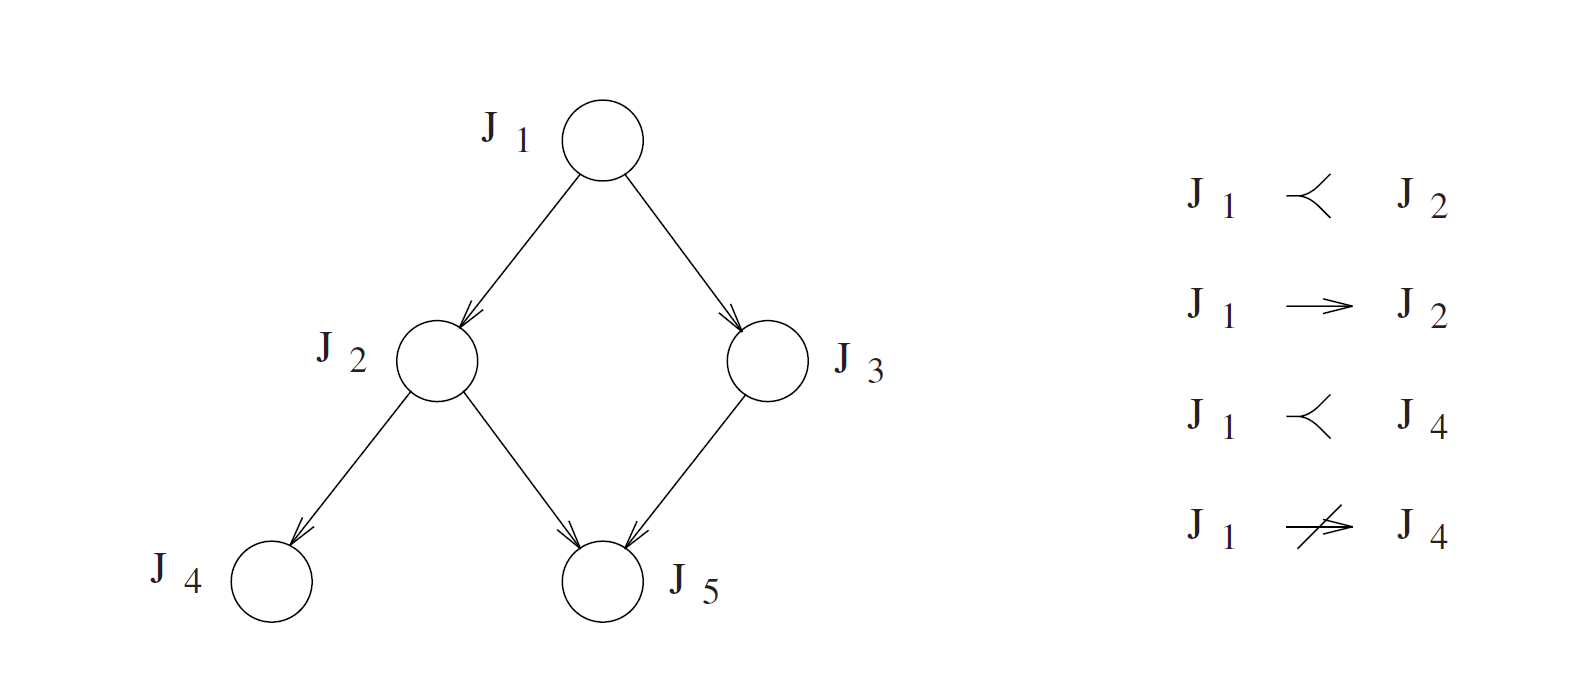
\includegraphics[width=\textwidth]{pictures/precedenzaTask.png}
    \caption{Relazione di precedenza tra 5 task}
\end{figure}
\noindent La notazione $J_a \prec J_b$ indica che il task $J_a$ è un predecessore di $J_b$, ovvero il grafo contiene un cammino orientato da $J_a$ a $J_b$.
\\
La notazione $J_a \rightarrow J_b$ indica che $J_a$ è un predecessore diretto di $J_b$, ovvero il grafo contiene un arco diretto da $J_a$ a $J_b$.
\\
I task senza predecessori vengono detti \textbf{task iniziali}, mentre quelli senza successori vengono detti \textbf{task finali}.
\subsubsection{Vincoli di mutua esclusione}
Dal punto di vista di un processo, una risorsa è una struttura software che può essere utilizzata dal processo per avanzare la sua esecuzione.
Una risorsa è detta \textit{privata} se è dedicata a un processo, altrimenti se può essere utilizzata da più processi è detta \textbf{condivisa}.
Per mantenere la correttezza del dato, molte risorse condivise non permettono l'accesso simultaneo da parte di task concorrenti, dunque richiedono la \textbf{mutua esclusione}.
La parte di codice che accede alla risorsa condivisa in mutua esclusione è detta \textbf{sezione critica}.
\begin{figure}[H]
    \centering
    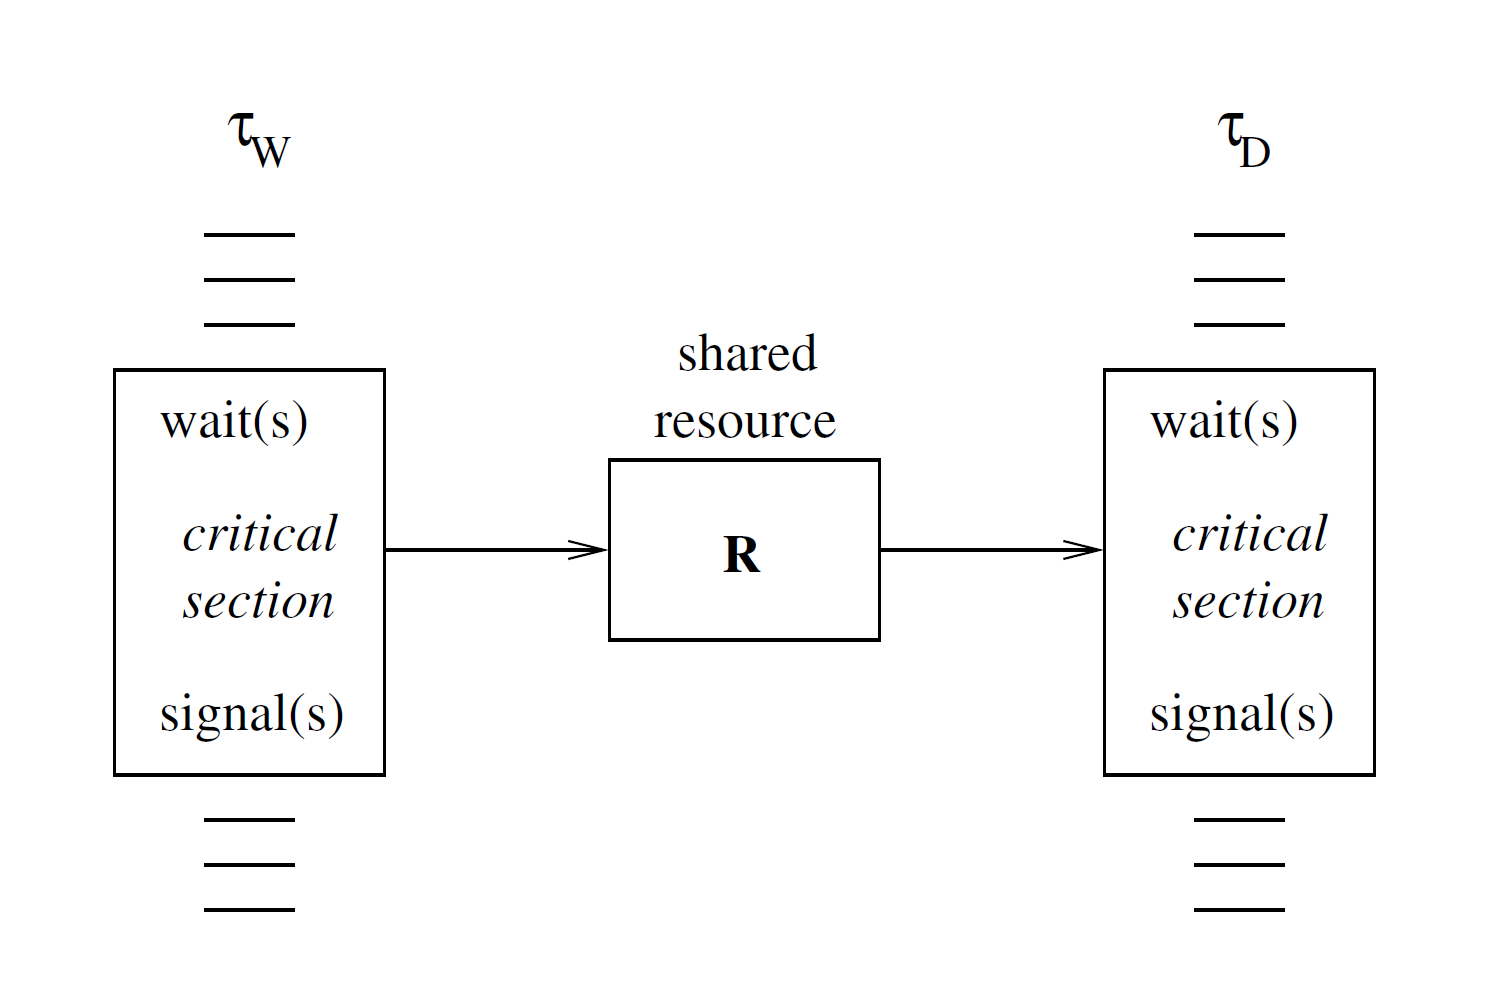
\includegraphics[width=0.60\textwidth]{pictures/strutturaSezioneCritica.png}
    \caption{Struttura di due task che accedono a una risorsa condivisa in mutua esclusione, tramite meccanismo di semafori}
\end{figure}
\begin{figure}[H]
    \centering
    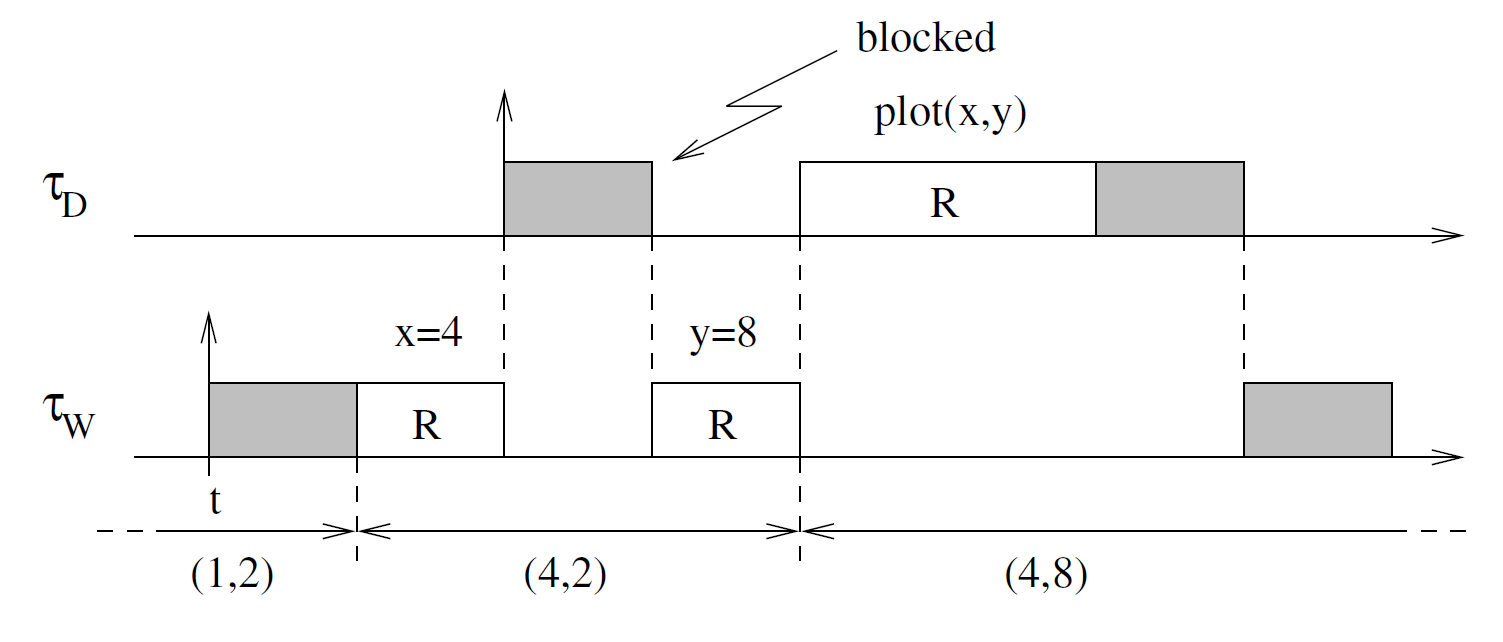
\includegraphics[width=0.75\textwidth]{pictures/schedulingCorsaCritica.png}
    \caption{Esempio di scheduling quando la risorsa è protetta da un semaforo}
\end{figure}
\begin{figure}[H]
    \centering
    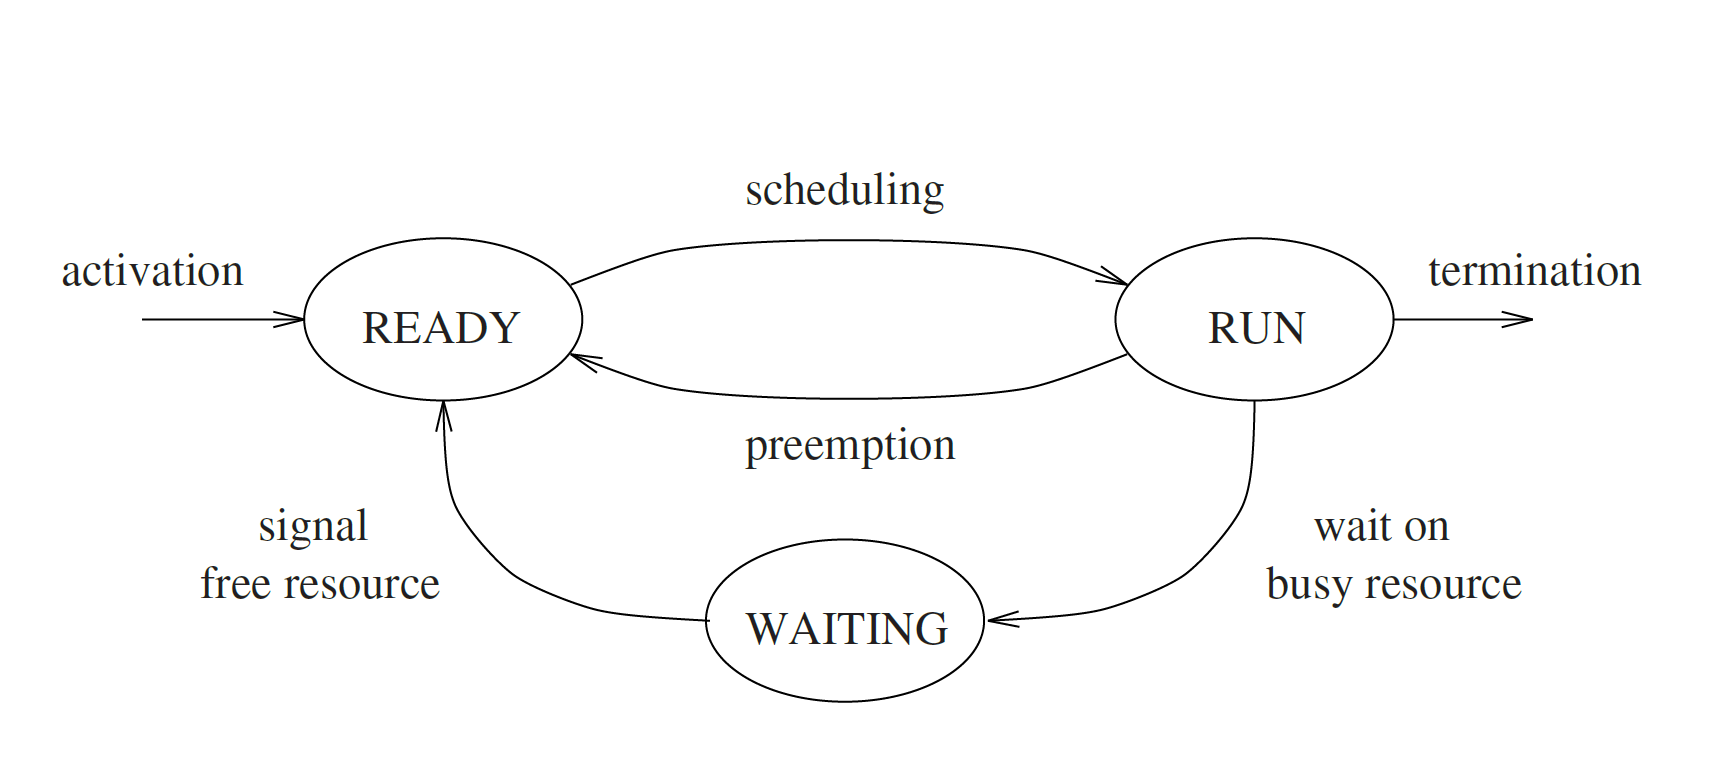
\includegraphics[width=0.75\textwidth]{pictures/cicloWait.png}
    \caption{Stato di wait causato da un vincolo sulle risorse}
\end{figure}
\noindent Quando un task è in attesa di una risorsa condivisa, si dice che \textit{bloccato} su quella risorsa.
Tutti i task bloccati su una stessa risorsa vengono messi in una \textbf{wait queue} associata a un semaforo che protegge la risorsa.
Quando un task in esecuzione utilizza la primitiva \textit{wait} su un semaforo bloccato, entra nello stato di \textbf{wait}, fino a quando un altro task non esegue la primitiva \textit{signal} che sblocca il semaforo.
Nota che quando un task lascia lo stato di wait non entra immediatamente nello stato di running, ma entra nello stato di ready, cosicché la CPU possa essere assegnata a un task con priorità più alta dall'algoritmo di scheduling.

\subsection{Classificazione di algoritmi di scheduling}
Le classi principali di algoritmi di scheduling sono:
\begin{itemize}
    \item \textbf{Preemptive vs. non preemptive}
    \begin{itemize}
        \item Preemptive: un task può essere interrotto in qualsiasi momento da un task con priorità più alta, secondo una policy di scheduling definita in precedenza.
        \item Non preemptive: un task una volta avviato deve essere eseguito fino al termine della sua esecuzione. Tutte le scelta di scheduling vengono effettuate quando il task termina la sua esecuzione.
    \end{itemize}
    \item \textbf{Static vs. Dynamic}
    \begin{itemize}
        \item Static: le decisioni di scheduling avvengono in base a un insieme di parametri che vengono definiti prima dell'attivazione dei task.
        \item Dynamic: le decisioni di scheduling avvengono in base a un insieme di parametri che possono essere modificati durante l'evoluzione del sistema.
    \end{itemize}
    
\end{itemize}
\end{document}
